\documentclass[12pt,toc=bib,toc=listof]{scrreprt}

\usepackage[autostyle=true]{csquotes}
\usepackage[ngerman]{babel} 
\usepackage[utf8]{inputenc}
\usepackage[T1]{fontenc}
\usepackage{lmodern}
\usepackage{setspace}
\usepackage{geometry}
\usepackage{graphicx}
\usepackage{xcolor}
\usepackage{booktabs}
\usepackage{amsmath}
\usepackage{caption}
\usepackage{subcaption}
\usepackage{authblk}
\usepackage[switch]{lineno}
\usepackage{apacite}
\usepackage{natbib}
\usepackage{listings}
\usepackage{xcolor}
\usepackage{tabularx}
\usepackage{enumitem}
\usepackage{multirow}
\usepackage{microtype}
\usepackage{cuted}
\usepackage{float}
\usepackage{stfloats}
\lstdefinestyle{systempromptstyle}{
    backgroundcolor=\color{gray!5},
    basicstyle=\ttfamily\small,
    breaklines=true,
    frame=single,
    rulecolor=\color{gray!30},
    captionpos=b,
    numbers=none,
    keywordstyle=\color{blue},
    commentstyle=\color{green!60!black},
    stringstyle=\color{purple},
    showstringspaces=false,
    inputencoding=utf8,
    extendedchars=true
    literate=%
        {Ö}{{\"O}}1
        {Ä}{{\"A}}1
        {Ü}{{\"U}}1
        {ß}{{\ss}}1
        {ü}{{\"u}}1
        {ä}{{\"a}}1
        {ö}{{\"o}}1
}


\usepackage{pdflscape}
\usepackage{pgfgantt}  
\usepackage{xcolor}

\definecolor{research}{RGB}{0,102,204}
\definecolor{development}{RGB}{0,153,76}
\definecolor{closure}{RGB}{204,0,0}
\definecolor{article}{RGB}{255,128,0}



\addto\captionsngerman{%
  \renewcommand{\bibname}{References}%
}

\usepackage{hyperref}
\hypersetup{
  pdftitle={Research_Project_Hefner_Hauptmann_\today},
  pdfauthor={Hefner, Robin;Hauptmann, Florian},
  colorlinks=true,
  linkcolor=black,
  citecolor=black,
  filecolor=black,
  urlcolor=black
}

\newcommand{\elqq}{``}
\newcommand{\erqq}{''}

\makeatletter
\renewcommand*{\@fnsymbol}[1]{\ensuremath{\number#1}}
\makeatother

\newcommand{\hhnsubject}{(172393) Research Project}
\newcommand{\hhnlecturer}{Prof. Dr. Petra Knaup}
\newcommand{\reprttopic}{Realistische Daten für ein lebendiges Lehre-KIS}

\newcommand{\reprtstudentAname}{Robin Hefner}
\newcommand{\reprtstudentAid}{206488}
\urldef{\reprtstudentAmail}\url{rohefner@stud.hs-heilbronn.de}

\newcommand{\reprtstudentBname}{Florian Hauptmann}
\newcommand{\reprtstudentBid}{225690}
\urldef{\reprtstudentBmail}\url{fhauptmann@stud.hs-heilbronn.de}

\usepackage[headsepline]{scrlayer-scrpage}
\pagestyle{scrheadings}
\clearscrheadfoot
\ihead{\hhnsubject: \reprttopic}
\ohead{\pagemark}
\renewcommand*{\chapterpagestyle}{scrheadings}
\renewcommand*{\chapterheadstartvskip}{}

\titlehead{
    
\includegraphics[width=0.3\textwidth]{./pictures/uni-hd.png}
    \hfill
    
\includegraphics[width=0.3\textwidth]{./pictures/hhn.png}
}
\subject{{\hhnsubject{}}}
\title{\reprttopic}
\author{
  \reprtstudentAname\thanks{\reprtstudentAid, \reprtstudentAmail} 
  \and 
  \reprtstudentBname\thanks{\reprtstudentBid, \reprtstudentBmail}
}
\publishers{Eingereicht bei \hhnlecturer}

\begin{document}

\pagenumbering{Roman} 
\selectlanguage{ngerman}
\maketitle
\setcounter{footnote}{0}

\newgeometry{left=30mm, top=25mm, right=15mm, bottom=25mm}
\tableofcontents
\newpage
\addchap{Abkürzungsverzeichnis}
\begin{description}
    \item[AI:] Artificial Intelligence
    \item[CGM:] Continuous Glucose Monitors
    \item[CIEL:] Columbia International eHealth Laboratory
    \item[CSV:] Comma-separated values 
    \item[EHR:] Electronic Health Record
    \item[EMR:] Electronic Medical Record
    \item[FHIR:] Fast Healthcare Interoperability Resources
    \item[GDPR:] General Data Protection Regulation
    \item[HIPAA:] Health Insurance Portability and Accountability Act
    \item[HIS:] Hospital Information System
    \item[HL7:] Health Level Seven International
    \item[IT:] Information Technology
    \item[JSON:] JavaScript Object Notation
    \item[LLM:] Large Language Model
    \item[PACS:] Picture Archiving and Communication System
    \item[PDF:] Portable Document Format 
    \item[PRISMA:] Preferred Reporting Items for Systematic Reviews and Meta-Analyzes
    \item[REST:] Representational State Transfer
    \item[SQL:] Structured Query Language
    \item[UI:] User Interface
    \item[XML:] Extensible Markup Language
\end{description}
\listoffigures
\listoftables
\newpage

\pagenumbering{arabic}
\onehalfspacing

\clearpage
\newgeometry{layout=letterpaper, 
paper=letterpaper, 
portrait, 
head=0.5in,
foot=0.5in,
top=1in, 
bottom=1in, 
left=0.75in, 
right=0.75in}
\setlength{\columnsep}{0.25in}
\pagestyle{plain}

\begin{otherlanguage}{english}
\begingroup
\setstretch{1.0}
\fontsize{10pt}{12pt}\selectfont

\makeatletter
\renewcommand*{\thesection}{\Roman{section}}
\setkomafont{section}{\normalfont\normalsize\bfseries}
\setkomafont{subsection}{\normalfont\fontsize{12pt}{12pt}\selectfont\bfseries}
\setkomafont{subsubsection}{\normalfont\fontsize{10pt}{10pt}\selectfont\bfseries}
\setkomafont{paragraph}{\normalfont\fontsize{10pt}{10pt}\selectfont\bfseries}

\renewcommand{\sectionlinesformat}[4]{%
  \ifstr{#1}{section}
  {\centering #3\MakeUppercase{#4}}
  {\@hangfrom{#3}{#4}}%
}
\renewcommand*{\sectionformat}{\thesection\quad}
\renewcommand{\bibsection}{\section*{\centering\MakeUppercase{\bibname}}}
\makeatother

\addcontentsline{toc}{chapter}{Wissenschaftlicher Artikel : Realistic data for a dynamic teaching HIS}

\twocolumn[{
  \begin{center}
    \setstretch{1.0}
    {\huge\bfseries Realistic data for a dynamic teaching hospital information system  \par}
    \vspace{1.5em}
    {\large Robin Hefner$^{1}$, Florian Hauptmann$^{1}$ \par}
    \vspace{1em}
    {\small $^1$Institute of Medical Informatics, Heidelberg University, Heidelberg, Germany;\par}
    \vspace{2em}
  \end{center}
}]

\textbf{Abstract --}
\textbf{Background:} Operational Hospital Information Systems (HIS) are essential for modern medical and medical informatics training. However, traditional educational HIS environments face legal and structural limitations, often relying on unpopulated databases or static datasets that fail to reflect dynamic, longitudinal clinical workflows.

\noindent\textbf{Objective:} Within the Heidelberg "studiKIS" project, this study aims to develop and systematically evaluate a methodology for providing realistic, privacy-compliant, dynamic data, including synthetic patient records and continuous wearable sensor streams, for a dedicated educational HIS.

\noindent\textbf{Methods:} A literature review on PubMed and IEEE Xplore (March 2026) identified state-of-the-art frameworks and integration standards. Core quality criteria were defined through six qualitative interviews with medical and IT experts. Prototypically, rule-based (Synthea) and LLM-based (Gemini 3.1 Pro) pipelines were engineered alongside a temporal ingestion script to simulate continuous hospital workflows in the open-source HIS Bahmni. Continuous glucose monitoring sensor streams were integrated via HL7 FHIR. Finally, 120 blinded patient records across three modalities (Real clinical data from MIMIC-III, Synthea, and LLM) were evaluated by clinical experts using a 5-point Likert scale and thematic qualitative analysis.

\noindent\textbf{Results:} Synthea-generated records achieved significantly higher ratings in longitudinal consistency (c2) compared to LLM profiles (p<0.001) and real data (p=0.027). No statistically significant differences were found for clinical plausibility (c1), chronological sequence (c3), and overall impression (c4). Qualitative analysis revealed distinct source-specific deficits: real data suffered from poor readability and chronological compression, Synthea datasets exhibited repetitive clinical patterns, and LLM data suffered from factual hallucinations and guideline violations. Empirical sensor streams were successfully visualized as trend graphs, though dynamic zooming and event annotation are natively lacking.

\noindent\textbf{Conclusion:} Providing dynamic, "living" clinical data via HL7 FHIR pipelines offers meaningful benefits over static teaching methods. Rule-based frameworks excel in life-span consistency but introduce rigid stereotypes, whereas LLMs generate flexible but often hallucinated records. Future work should focus on scalable translation scripts for rule-based systems and knowledge-grounded AI architectures (such as RAG and multi-agent critic frameworks) to eliminate clinical inaccuracies.
    
    \smallskip
    \smallskip
    
\noindent\textbf{Keywords} -  Hospital Information System; HIS; Synthetic Clinical Data; Electronic Health Record; HL7 FHIR; Synthea; Large Language Models; Medical Sensors; Medical Education


\section{Introduction}
Hospital Information Systems (HIS) are the core infrastructure of the modern public health system. Accordingly, the development of a suitable educational HIS for academic training in human medicine and medical informatics is essential. To create a fully functional and realistic educational HIS, the project investigates the generation of structured, longitudinal synthetic clinical data alongside the integration of continuous sensor data streams from medical wearables.

The ability to proficiently navigate and use operational HIS is a fundamental competency in modern medical education \citep{BICHELFINDLAY2023104908}. As healthcare becomes increasingly digitized, students must not only understand traditional clinical workflows but also learn to manage heterogeneous data formats, use various technical interfaces, and evaluate the growing role of patient-generated health data in the treatment context \citep{healthcare13030329}. Practical, hands-on experience with realistic, evolving patient histories and continuous physiological monitoring is therefore important to effectively prepare future physicians for the complexities of modern, data-driven patient care \citep{Mohan2016-qn}.

Despite this educational necessity, traditional training environments face significant structural and legal limitations. The widespread use of authentic electronic health records (EHRs) is strictly restricted by data privacy regulations such as the General Data Protection Regulation (GDPR) and the Health Insurance Portability and Accountability Act (HIPAA) \citep{Chen2021-ji}. Consequently, academic HIS often rely on unpopulated databases or static synthetic datasets \citep{choi2021}. These static approaches represent merely a cross-section of a specific point in time, failing to adequately reflect the dynamic, longitudinal nature of clinical workflows or the continuous evolution of clinical parameters required to analyze disease progressions \citep{Majumder2017-tg}.

To bridge this pedagogical gap, this project aims to develop a methodology for providing dynamic data for a dedicated educational HIS within the Heidelberg \enquote{studiKIS} project. The primary objective is to synthetically generate structured clinical data that continuously evolves over time, enabling students to observe and analyze realistic, longitudinal treatment trajectories. Furthermore, the project integrates real-world sensor data to teach students how to process diverse data formats and technical interoperability standards, such as HL7 FHIR. By engineering this dynamic data pipeline and systematically evaluating its clinical plausibility, the project yields a privacy-compliant, highly realistic simulation environment that bridges the gap between theoretical knowledge and practical clinical application.

\section{Background}
\subsection*{Synthetic Clinical Data}

\subsection*{Bahmni}

\subsection*{Virtual HIS}

\subsection*{Synthea}




\section{Methods}
\label{sec:methods}

This section describes the methodological framework employed to evaluate synthetic clinical data generation and the integration of sensor data into the Heidelberg studiKIS. The research followed a structured four-phase approach.

\subsection*{Literature Review}
A comprehensive literature review was conducted to identify and analyze current state-of-the-art approaches, focusing on studies that addressed at least one of the following two primary domains:
\begin{enumerate}
    \item \textbf{Synthetic Clinical Data Generation:} Investigation of Large Language Models (LLMs) and autonomous agent systems, encompassing both classical rule-based architectures and modern LLM-based agents for the creation of longitudinal patient records.
    \item \textbf{Sensor Data Integration:} Identification of existing standards and protocols for exporting medically relevant data and integrating real-time sensor data from medical devices and wearables into Hospital Information Systems (HIS).
\end{enumerate}
\subsubsection*{Eligibility criteria}
Papers were included if they met at least one of the following two criteria:
\begin{enumerate}
    \item Papers were included if they utilized LLMs, Generative AI, or model-based approaches employing state machines specifically for the purpose of generating synthetic clinical health data.
    \item The papers had to include the collection of sensor data and their integration in a HIS or the Electronic Health Records (EHR). Paper were excluded, when they only collected sensor data to train machine learning algorithms without the integration into the HIS or EHR.
\end{enumerate}
\subsubsection*{Information sources}
Literature for this research project was systematically retrieved from two primary electronic databases: PubMed and the IEEE Xplore Digital Library. These sources were selected to ensure a comprehensive coverage of both the clinical and technical dimensions of the research topics.

PubMed was utilized as the principal source for identifying peer-reviewed literature within the life sciences and biomedical domain. It provided essential insights into clinical workflows and the medical requirements for synthetic patient data generation, as well as the practical application of sensor data integration within healthcare environments.

To address the high-level technical and architectural challenges of the project, the IEEE Xplore Digital Library was employed. Furthermore, IEEE Xplore provided the necessary technical depth regarding the algorithmic approaches and architectural frameworks required for the automated generation of synthetic clinical datasets and the seamless integration of sensor data into existing Hospital Information Systems.

The search was conducted during March 2026.

\subsubsection*{Search Strategy}
\begin{enumerate}
    \item For IEEE Xplore and PubMed the following search string was used: ((\enquote{synthetic data generation} OR \enquote{synthetic clinical data} OR \enquote{synthetic data} OR \enquote{synthetic patient} OR \enquote{synthetic patient data} OR \enquote{synthetic EHR} OR \enquote{Synthea})
    \textbf{AND}
    (\enquote{large language models} OR \enquote{LLM} OR \enquote{generative AI} OR \enquote{autonomous agents} OR \enquote{agent-based} OR \enquote{machine learning})
    \textbf{AND}
    (\enquote{clinical workflows} OR \enquote{patient history} OR \enquote{medical records} OR \enquote{case vignettes} OR \enquote{longitudinal} OR \enquote{simulated patients}))
    
    No restrictions were applied regarding publication year or language.
    
    \item The search string used for PubMed was: ((\enquote{Hospital Information Systems} [MeSH] OR \enquote{Electronic Health Records} [MeSH]) 
    AND (\enquote{sensor*} OR \enquote{sensor data} OR \enquote{wearable*}) 
    AND (\enquote{storage} OR \enquote{archiving} OR \enquote{persistence} OR \enquote{NoSQL} OR \enquote{SQL} OR \enquote{Time-series database} OR \\\enquote{openEHR} OR \enquote{FHIR} OR \enquote{repository})) 
    NOT (\enquote{Blockchain} OR \enquote{Security} OR \enquote{Cryptography} OR \enquote{Privacy Preservation} OR \enquote{Cybersecurity}).
    
    The search string used for IEEE Xplore was identical, only the \textit{[MeSH]} filters were removed, as they do not exists in IEEE Xplore.
    
    Only articles in the language German and English were considered, however no restrictions were applied regarding the publication year.
\end{enumerate}
\subsubsection*{Synthesis methods}
\begin{enumerate}
    \item To evaluate the current landscape of synthetic clinical data generation, a quantitative analysis was performed. Each included paper was systematically categorized based on the underlying technology or framework used for data synthesis.
    Each study was manually reviewed to identify the primary synthesis engine.

    \item A second quantitative analysis examined current approaches for integrating sensor data into HIS or EHR systems. For each paper, we extracted and compared the transmission protocols, the interfaces utilized, and whether the communication with the HIS relied on a push or pull mechanism.
\end{enumerate}

\subsection*{Definition of Quality Criteria}
To guarantee the pedagogical and technical utility of the synthesized datasets for medical informatics education, a formal set of quality requirements was defined. Methodologically, a structured interview guideline was designed to target medical, information technology, and didactic quality metrics. Using this instrument, five qualitative, target-group-adapted interviews were conducted with a cohort consisting of four medical experts and one specialized IT professional. A unifying selection criterion for all five domain experts was their extensive practical experience in academic teaching. Qualitative analysis of the interview transcripts yielded four core dimensions of data quality: clinical plausibility (the medically logical interplay of symptoms, diagnoses, and treatments), longitudinal consistency (uninterrupted, coherent progression of chronic conditions over extended periods), chronological-logical sequence (realistic time intervals between clinical events), and overall impression (the global synthesis dictating student acceptance and didactic value).

\subsection*{Prototypical Implementation and Dataset Generation}
The practical phase was executed through two parallel implementation workflows: rule-based generation utilizing a modified simulation framework and agentic generation using Large Language Models, followed by their ingestion into the Hospital Information System (HIS).

\subsubsection*{Rule-Based Generation via Synthea}
Patient generation utilized the open-source Synthea repository along with its official documentation. Three key structural hurdles were addressed during implementation. First, to adapt Synthea’s native North American healthcare and demographic profiles to a European context, the repository was forked to incorporate German localized properties, introducing German names, street addresses, cities, hospitals, and health insurance entities. Second, because Synthea natively generates complete, lifelong patient histories which lack realism for an active, acute HIS environment, the resulting FHIR bundles were programmatically sliced into discrete transactions. This allows the import process to be halted at a specific clinical cut-off point. Third, to prevent an unmanageable, exponential proliferation of virtual clinicians within the HIS database—a native characteristic of Synthea—a provider-pooling strategy was designed. A custom script was conceptualized to scan the FHIR bundles and systematically substitute Synthea-generated clinicians with a fixed pool of pre-existing HIS users assigned to five specialized departments (Cardiology, Neurology, Chest Pain Unit, Stroke Unit, and Neurological Rehabilitation). Due to time constraints, this was verified via a manually curated pilot patient dataset where clinical observations were mapped to the predefined provider pool.

\subsubsection*{Large Language Model Generation}
An agentic data synthesis pipeline was engineered by developing advanced prompts for the Gemini 3.1 Pro (High) model to generate structured clinical records directly as FHIR bundles. To mitigate the critical hurdle of clinical hallucinations and inconsistent disease trajectories, the model was supplied with a restricted, reference taxonomy of valid diagnoses and medications. This significantly enhanced the clinical plausibility and internal coherence of the output. Formatting inconsistencies within the generated JSON-based FHIR bundles were resolved by extending the prompt architecture with explicit OpenMRS-compatibility criteria and strict structural formatting rules.

\subsubsection*{System Integration and HIS Ingestion}
The generated synthetic records were ingested into the target HIS via its native FHIR API module. Ingestion was impeded by several technical boundaries, most notably the insufficient documentation of the Bahmni FHIR module, which required empirical reverse-engineering of accepted endpoints and data structures. Semantic gaps caused by missing concepts within the HIS database were resolved by integrating the comprehensive CIEL concept dictionary. 

Furthermore, the structural complexity of Synthea's full FHIR bundles led to repeated architectural rejections by the HIS. A prescriptive troubleshooting strategy, consisting of loading datasets, analyzing error logs, programmatically stripping non-compliant fields, and re-attempting the import, revealed deep scalability limitations due to unpredictable fields in subsequent simulation runs. Consequently, the ingestion pipeline shifted its primary focus to the highly compliant LLM-generated FHIR bundles.

To automate laboratory value ingestion, which natively requires a complex two-stage process in Bahmni (order placement and laboratory information system callback), an initial Python script was developed to simulate HTTP network requests captured from UI interactions. Because linking laboratory orders to patient IDs occurred dynamically via the UI URL structure rather than a discrete payload, a fallback mechanism utilizing direct SQL database queries was implemented. 

In parallel to these synthetic workflows, real-world physiological sensor data was integrated into the ingestion pipeline. This empirical dataset was gathered from three human participants who tracked their continuous glucose levels over a duration of two weeks utilizing the FreeStyle Libre 3 sensor. While the initial script-based database ingestion method succeeded in appending bulk data, it could not backdate historical timestamps. The final architecture resolved this temporal limitation for both laboratory measurements and continuous glucose streams by identifying the exact, low-level FHIR Observation schema accepted by the HIS. This allowed historical trends and high-frequency sensor data points to be imported seamlessly via the regular FHIR interface as general observations visualized within the system's native trends dashboard.

\subsubsection*{Dynamic Temporal Data Ingestion}
To transform the static database into a \enquote{living} clinical environment, a temporal ingestion pipeline was deployed. A custom Python script parses the synthesized clinical data into individual, chronological FHIR transactions and persists them within a local SQLite database, appending a target \enquote{Scheduled-Time} attribute to each entry. A secondary script executes continuously as a cronjob on the central HIS server, querying the SQLite database at regular intervals and dynamically executing the FHIR import for all transactions whose scheduled execution time has been reached.

\subsection*{Evaluation of the Investigated Approaches}
To objectively measure the efficacy, complexity, and structural quality of the synthesized datasets against real-world clinical baselines, a rigorous evaluation framework was established.

\subsubsection*{Data Cohort Selection}
The evaluation matrix incorporates data from three distinct technological dimensions: rule-based simulation (Synthea), agentic generative models (LLM), and real clinical records. The real-world baseline was derived from anonymized patient records extracted from the public MIMIC-III dataset. To ensure statistical balance, a uniform 40/40/40 split was enforced, yielding a total evaluation sample size of 120 unique patient records.

\subsubsection*{Blinded Homogenization and Presentation Pipeline}
To eliminate evaluative bias and ensure a strict double-blind testing protocol, all records had to be presented in an identical, visually indistinguishable format. Because direct HIS visualization was unfeasible due to the Synthea ingestion constraints, a universal PDF-based rendering pipeline was engineered, preventing evaluators from reviewing raw FHIR code blocks.

Two specialized pipeline scripts were implemented. The first script extracts and normalizes the highly heterogeneous source data, including Synthea's tabular CSV exports and the JSON-based FHIR bundles from the LLM and MIMIC-III sources, into an identical, intermediate CSV template. The second script parses this standardized template to generate structurally uniform PDF documents. To mask the complete demographic anonymity of the real clinical baseline, which lacked names and addresses, records were algorithmically populated with pseudo-randomized German identities. These identities were cross-referenced with the patient's recorded biological sex to prevent logical contradictions. To account for variations in information depth across the sources (e.g., Synthea’s native generation of insurance and billing metrics), the PDF display layout was strictly homogenized to feature five clinical dimensions: allergies, diagnoses, medications, procedures, and laboratory/vital signs.

\subsubsection*{Evaluation of Patient Data}
Data collection was facilitated by developing a password-protected, web-based application split into a dual-pane interface. The left pane dynamically renders the randomized patient PDF, while the right pane exposes the scoring instruments composed of 5-point Likert scales alongside open-ended qualitative feedback fields. To control for observer bias, three anonymized evaluator profiles were generated, and their credentials were distributed to the participating physicians by an external, blinded coordinator. The web application enforces data integrity by preventing duplicate evaluations, caching session progress persistently within a cloud database, and automatically filtering out completed records until the 120-case matrix is fulfilled. Standardized execution was maintained via a comprehensive, written evaluation protocol provided to all participating experts.

\subsubsection*{Evaluation of Sensor Data Integration}
Unlike the algorithmically synthesized patient trajectories, the integrated sensor data streams were not subjected to the predefined qualitative and didactic evaluation criteria. Because these data streams consist of authentic, real-world physiological data points rather than generated outputs, evaluating their internal clinical plausibility, logical consistency, or overall structural generation artifacts was redundant. 

Instead, the evaluation framework for this domain targeted the structural ingestion limits and frontend display possibilities within the Heidelberger studiKIS environment. The primary focus of this assessment was to evaluate how effectively the software infrastructure visualizes high-frequency continuous data. Specifically, the system was scrutinized on its capacity to handle, render, and maintain the granular data points produced by the FreeStyle Libre 3 sensors over a continuous two-week interval without compromising dashboard performance or user-end scannability.


\section{Results}
\subsection*{Literature Review and Synthesis Findings}
The systematic literature review identified a total landscape of relevant literature across both primary domains:
\begin{itemize}
\item \textbf{Synthetic Data Generation:} The analyzed landscape is primarily shaped by Large Language Models (LLMs) and Transformers (n=9), followed by Generative Adversarial Networks (GANs) used for tabular and image data (n=4), agent-based simulation via Synthea (n=2), and emerging probabilistic approaches such as diffusion and interactive frameworks (n=2).
\item \textbf{Sensor Data Integration:} The analysis revealed a clear dominance of the HL7 FHIR standard (n=11), while classical REST interfaces for data transmission were utilized in only a minority of studies (n=3). Notably, none of the investigated papers described continuous data streaming into the HIS; instead, integration was exclusively achieved via batch-processing methodologies using targeted server pull mechanisms.
\item \textbf{Extracted Literature Requirements:} Core requirements extracted from literature encompass seven distinct domains: statistical fidelity (e.g., high-dimensional disease codes reaching correlation probabilities of R2>0.9) \citep{chen_generating_2025} \citep{theodorou_synthesize_2023}, structural integrity (hierarchical consistency and modeling informative missingness)\citep{josling_novel_2026}, temporal dynamics (realistic inter-visit gaps) \citep{josling_novel_2026} \citep{theodorou_synthesize_2023}, clinical utility (validated via the \enquote{Train-Synthetic-Test-Real} framework)\citep{theodorou_synthesize_2023} \citep{jung_clinical_2025}, data privacy (differential privacy to mitigate re-identification risks)\citep{tsao_health_2023} \citep{hahn_contribution_2022} \citep{chen_generating_2025}, governance/ethics (adherence to FAIR and CARE principles)\citep{tsao_health_2023}, and active bias mitigation\citep{theodorou_synthesize_2023}.
\end{itemize}

\subsection*{Defined Quality Criteria from Expert Interviews}
Six qualitative interviews were successfully completed with a balanced cohort consisting of three medical experts and three specialized IT professionals. Qualitative analysis of the interview transcripts successfully yielded four established core dimensions of data quality for academic teaching:
\begin{enumerate}
\item \textbf{Clinical Plausibility:} The medically logical interplay of symptoms, diagnoses, and treatments, ranging from error-free standard therapies to plausible medical errors.
\item \textbf{Longitudinal Consistency:} Uninterrupted, coherent progression of chronic conditions and follow-up examinations over extended periods without illogical jumps.
\item \textbf{Chronological-Logical Sequence:} Realistic time intervals between clinical events (e.g., from initial diagnosis through intervention to follow-up care).
\item \textbf{Overall Impression:} The global synthesis of the patient record dictating student acceptance and final didactic value.
\end{enumerate}

\subsection*{Prototypical Implementation and Pipeline Performance}
The practical implementation phase yielded functioning technical pipelines with distinct outcomes across the rule-based simulation, the generative AI workflows, and the empirical sensor data integration.

\subsubsection*{Synthea Customization and Limitations}
A functioning workflow was established to generate patient collectives in the localized FHIR format. However, implementation was impeded by significant technical and temporal constraints:
\begin{itemize}
\item Due to time restrictions, the provider-pooling strategy could not be fully developed into an automated script. It was instead verified via a manually curated pilot patient dataset where clinical observations were mapped to a predefined provider pool across five specialized departments.
\item The structural complexity of Synthea's full FHIR bundles led to repeated architectural rejections by the HIS. An iterative troubleshooting approach (analyzing error logs and programmatically stripping non-compliant fields) proved unscalable for subsequent simulation runs due to unpredictable fields. Combined with semantic gaps and insufficient documentation of the Bahmni FHIR module, the ingestion pipeline for rule-based data encountered deep scalability limitations and was ultimately deprioritized.
\end{itemize}

\subsubsection*{LLM Pipeline and Synthetic Record Ingestion Results}
Advanced prompting of the Gemini 3.1 Pro (High) model successfully minimized clinical hallucinations and formatting inconsistencies, resulting in highly compliant JSON-based FHIR bundles. Because of the scalability issues encountered with Synthea's complex bundles, the automated ingestion pipeline shifted its primary focus to these LLM-generated records. Integrating the comprehensive CIEL concept dictionary successfully resolved semantic gaps caused by missing concepts in the HIS database. 

\subsubsection*{Integration and Visualization of Empirical Sensor Data}
The continuous glucose sensor streams gathered from the four human participants were successfully parsed and integrated into the HIS database via the standard FHIR interface. By modeling the high-frequency time-series data as low-level FHIR Observation resources, the pipeline completely bypassed the system's standard clinical ordering workflows. Consequently, the granular temporal datasets were successfully processed by the backend and visualized dynamically within the system's native frontend trends dashboard, fulfilling the core requirements for real-time data representation in the educational environment.

\subsection*{Evaluation Dataset and Platform Generation}
The implemented rendering and presentation pipeline successfully generated a structurally uniform evaluation dataset:
\begin{itemize}
\item A total sample size of 120 unique, visually indistinguishable patient records was successfully compiled based on a precise 40/40/40 split (40 Synthea-simulated, 40 LLM-generated, and 40 real clinical records from the MIMIC-III baseline).
\item The final PDF documents successfully harmonized the varying information depths by restrictively rendering exactly five clinical dimensions: allergies, diagnoses, medications, procedures, and laboratory/vital signs.
\item The password-protected web application was successfully deployed, featuring the complete dual-pane evaluation interface. The system successfully enforces data integrity by persistently caching session progress in a cloud database, preventing duplicate evaluations, and dynamically managing the 120-case matrix for the blinded evaluators.
\end{itemize}

\section{Discussion}
\subsection*{Interpretation of Findings}
\subsubsection{Interpretation of Quality Criteria}
Comparing the literature and interview findings reveals shared core requirements for synthetic data evaluation but divergent priorities regarding its application. Both sources align on the need for temporal and clinical coherence, as the literature focuses on temporal dynamics and clinical utility \citep{josling_novel_2026, theodorou_synthesize_2023, jung_clinical_2025} that match the experts demands for chronological sequencing, longitudinal consistency, and clinical plausibility. Furthermore, the experts requirement for interoperability standards like HL7 FHIR mirrors the literature's emphasis on governance, ethics, and FAIR principles \citep{tsao_health_2023}. 

However, their primary evaluation metrics differ. While the literature prioritizes quantitative metrics such as statistical fidelity \citep{chen_generating_2025, theodorou_synthesize_2023}, structural integrity\citep{josling_novel_2026}, and mathematical privacy guarantees \citep{tsao_health_2023, hahn_contribution_2022, chen_generating_2025}, the interview results focus on qualitative and pedagogical utility for academic teaching. For educational purposes, experts prioritize narrative coherence, realistic clinical elements like medical errors, and adaptable case complexity. Consequently, while statistical parameters ensure technical validity and privacy, educational utility depends strictly on narrative realism and didactic flexibility.

\subsubsection{Interpretation of Quantitative and Qualitative Group Differences in Patient Data}
Statistically significant differences were limited to criterion $c2$ (Longitudinal Consistency), where Synthea-generated patient data outperformed LLM-generated records and demonstrated a positive trend against real-world data. These results may be attributed to Synthea's underlying generative framework, which is designed to simulate a patient's entire lifespan, beginning at birth, tracking all clinical encounters, and concluding at death \citep{synthea}. Consequently, longitudinal consistency is inherent to these records. In contrast, LLM-based patient profiles contained fewer encounters, observations, and diagnoses. Furthermore, while real-world data captured higher encounter volumes, they spanned a shorter historical duration. These factors likely explain Synthea’s significant improvement over LLM profiles and its positive, although non-significant, trend against real-world benchmarks.

However, this comprehensive data generation model also introduced a major point of criticism in the qualitative findings. Evaluators noted that Synthea-generated records exhibited repetitive patterns, such as an overrepresentation of dental cases. This artifact reflects the lifespan-simulation methodology, where frequent, routine dental checkups naturally outnumber visits to hospitals.

For criteria $c1$, $c3$, and $c4$, the generated data were statistically comparable to each other and to authentic records. However, a wide score distribution across all modalities indicated high variance and low inter-rater reliability. Qualitative observations explain this variance: real-world records suffered from poor readability and unspecific coding, likely stemming from localized hospital abbreviations. Synthea records exhibited repetitive patterns and occasional lapses in clinical plausibility, and LLM data contained factual errors and hallucinations. Evaluators most likely prioritized these distinct deficits differently based on their clinical focus, penalizing structural disorganization, logical inconsistencies, or hallucinations with varying severity, resulting in low inter-rater reliability.

\subsubsection{Interpretation of Sensor Data Visualization Quality}
The Bahmni patient dashboard natively renders assigned laboratory values as continuous graphs. By mapping the sensor data to an appropriate concept and importing them via the FHIR interface, the streams were successfully visualized, satisfying core expert requirements for real-time data representation. Furthermore, Bahmni automatically highlights out-of-range values, provided the range is defined in the concept. However, this flagging mechanism appears to be persisted at the database level during data ingestion rather than evaluated dynamically at runtime during visualization. Consequently, values imported via the FHIR interface lacked out-of-range indicators despite breaching the defined ranges, whereas manually entered values were flagged appropriately. Incorporating range parameters within the FHIR payload might circumvent this barrier, but due to time constraints, this hypothesis could not be verified.

Consequently, the platform inherently satisfies the \textit{Graphical Trend Visualization} criterion and could potentially satisfy \textit{Anomaly Highlighting}, provided programmatic triggering can be achieved via the ingestion pipeline. However, the remaining two criteria, \textit{Adaptive Contextual Granularity} and \textit{Temporal Event Annotation}, are not supported out of the box. Prospective enhancements are detailed in Section Advanced UI Component Engineering for Sensor Stream Dashboarding.

\subsection*{Limitations}
\subsubsection{Literature Review}
To ensure comprehensive coverage of both the clinical and technical dimensions of the research, the literature review focused on two primary databases: PubMed and IEEE Xplore. While a structured methodology was applied, the search did not strictly adhere to systematic review standards or full PRISMA guidelines. Because the primary objective was the technical integration of data into a virtual HIS, the literature search served only to establish a functional baseline. Consequently, expanding the database selection and executing a full systematic review fell outside the project's scope.

\subsubsection{Limitations regarding Data Completeness}
Due to time constraints, 90 patient records were not evaluated by the third reviewer, introducing a risk of verification bias. However, given the fixed project timeline and the availability of two complete evaluation rounds for the entire sample, the analysis was proceeded. 

\subsubsection{Technical Limitations}
Because Synthea-generated patient records were too structurally complex for direct HIS import, an initial troubleshooting strategy was designed to analyze error logs and programmatically strip non-compliant fields. However, this approach was quickly deemed too time-intensive and raised scalability concerns, as manually auditing individual profiles cannot guaranty compatibility across subsequent patient records. Nonetheless, given the significant performance advantage observed for Synthea data regarding criterion $c2$ over LLM alternatives, developing a translation script to map Synthea's output to an HIS-compliant FHIR schema may present a key area for future work. Such an integration pipeline requires careful calibration. A naive truncation technique that blindly removes non-compliant fields risks degrading the clinical realism that drove Synthea’s performance metrics. Hence, it may be necessary to develop alternative import strategies rather than simple data truncation to preserve dataset integrity.

Tied to the complexity of the Synthea files was the current inability of creating a script, which replaced all newly generated Synthea providers to a predefined set of existing HIS clinicians. However, manual validation confirmed that provider replacement was successful within simplified Synthea profiles, and the Bahmni user interface correctly displayed the assigned personnel alongside their corresponding diagnoses. Consequently, while an automated provider-mapping script is theoretically possible, its utility is dependent on the script adapting the Synthea generated FHIR file to a FHIR structure accepted by Bahmni.

In contrast, generating compliant FHIR structures for LLM-generated patient profiles is significantly more straightforward, as the output schema can be strictly enforced through targeted prompting. A limitation remains the reproducibility of LLM outputs across different model versions. Nevertheless, the detailed prompt architecture is expected to minimize variance when deploying alternative models, preserving the framework's generalizability.

\subsection*{Future Work}
\label{sec:further_research}
Based on the technical challenges, qualitative findings, and architectural trade-offs, these four areas for future research have been defined:

\subsubsection{Automated Ingestion and Interoperability Pipelines for Rule-Based Simulation}
Future work should develop a scalable translation script to map native Synthea FHIR bundles to HIS-accepted profiles. This pipeline must address two architectural gaps:
\begin{itemize}
    \item \textbf{Dynamic Concept Harvesting:} Active database synchronization using the CIEL concept dictionary to programmatically inject missing clinical concepts into the HIS backend prior to ingestion.
    \item \textbf{Automated Provider Pooling:} A script to map dynamically generated virtual clinician identities to a fixed pool of pre-existing HIS users across specialized departments.
\end{itemize}
Future studies must evaluate the trade-off between structural simplification and medical realism to ensure that system compatibility does not compromise clinical complexity.

\subsubsection{Knowledge-Grounded Architectures for Generative AI}
To mitigate clinical hallucinations and guideline violations in LLM-generated records, future architectures should transition to knowledge-grounded generation:
\begin{itemize}
    \item \textbf{Retrieval-Augmented Generation (RAG):} Coupling the generative engine with a vector database of localized clinical guidelines to ground probabilistic patient transitions in authentic pathways.
    \item \textbf{Multi-Agent Critic Frameworks:} A dual-agent system where a generative model synthesizes the history, while a specialized ``Clinical Critic'' agent verifies medical facts, units, and chronologies prior to database export.
\end{itemize}

\subsubsection{Advanced UI Component Engineering for Sensor Stream Dashboarding}
To address limitations in interactive granularity and contextual layout within the sensor dashboard, the following frontend extensions are proposed:
\begin{itemize}
    \item \textbf{Interactive Frontend Scaling:} Zoom and pan components to adjust temporal resolutions directly within the browser, avoiding database downsampling or manual reloads.
    \item \textbf{Temporal Event Annotation:} A mechanism to anchor discrete lifestyle metrics (e.g., dietary intake) onto tracking graphs, allowing students to correlate behaviors with physiological responses.
\end{itemize}
Implementing these features in Bahmni might require core codebase alterations, posing maintainability risks during framework updates. This could lead to either repetitive manual code synchronization upon every release or upstream adoption by the core Bahmni development team, so that the changes persist in upcoming versions. Due to the lack of long-term sustainability for local customizations, evaluating alternative virtual HIS platforms that natively support these requirements may be necessary.

\subsubsection{Improving the Continuous Clinical Workflow}
By using a two-step approach, which partitions patient records into individual transactions and executes imports via a cron job at scheduled times, successfully simulates a real-world clinical workflow. However, determining appropriate temporal intervals between distinct encounters and diagnoses remains an open question, as does identifying the optimal baseline for the initiation of a patient record. 

Because Synthea-generated profiles track an individual’s history from birth, subsequent clinical events are distributed across decades. Simulating continuous ingestion from birth is practically unfeasible, as real-time execution would mirror an actual lifespan. A more viable alternative could involve a hybrid ingestion strategy: statically importing a historical baseline of encounters and diagnoses, followed by dynamic, continuous workflows. Nevertheless, the temporal fidelity of synthetic encounters requires further evaluation. While criterion $c3$ (Chronological-Logical Sequence) evaluates this progression in this article, neither Synthea nor LLM-generated datasets currently excel in this domain. Consequently, further research is required to optimize chronological logic before deploying these synthetic profiles in medical education.

Alternatively, to maximize control over educational datasets, course instructors could predefine patient records aligned directly with specific lesson plans. Instructors would configure the \textit{Scheduled-Time} attribute to dictate exactly when a virtual patient is imported with the HIS. This workflow could be driven by a dedicated web application integrated with the ingestion database, allowing the cron job to extract these targeted encounters. Developing and evaluating such a pedagogical management platform could be the focus of a subsequent study.

\subsubsection{Methodological Scaling and Multi-Reviewer Validation}
Finally, to address the risk of verification bias stemming from the incomplete third evaluation round of 90 datasets, future evaluation cycles must enforce full multi-reviewer coverage across the entire case matrix. Additionally, research should systematically evaluate inter-rater disagreement to understand how subjective expert priorities influence the validation of synthetic clinical data.

\section{Conclusion}
This research project demonstrates the feasibility of generating synthetic patient data through rule-based approaches using Synthea and generative AI approaches using LLMs. Synthea-generated records showed significant improvements over LLM generated records concerning longitudinal consistency and a positive trend over real-world patient data. By sequentially importing these records into a HIS using HL7 FHIR standards, the system simulates the continuous nature of real-world clinical documentation. Additionally, continuous data streams from wearables were imported into the HIS and displayed using the patient's native dashboard. These dynamic structures allow students to analyze realistic disease progression and patient-generated data without privacy risks.

Despite these advantages, the current implementation has several limitations. Rule-based profiles from Synthea produced repetitive patterns, and their FHIR bundles were rejected by the HIS due to structural complexity. Conversely, Large Language Models generated simpler, compatible FHIR data but suffered from broken timelines and clinical hallucinations. Furthermore, the sensor integration lacked interactive frontend features like temporal scaling, and the evaluation was limited by low inter-rater reliability.

Future research should focus on technical and methodological refinements. Key priorities include developing scalable translation scripts to map complex rule-based outputs to HIS-compliant schemas, alongside implementing knowledge-grounded AI architectures, such as Retrieval-Augmented Generation and multi-agent frameworks, to actively enforce guideline compliance and eliminate hallucinations. Additionally, dedicated frontend engineering is required to enable dynamic downsampling and event marking within the sensor dashboard. Addressing these technical barriers and expanding future evaluations to full multi-reviewer validation will help establish reliable, dynamic simulation environments for medical education.

\bibliographystyle{apacite}
\bibliography{references} 

\endgroup
\end{otherlanguage}

\clearpage
\onecolumn
\restoregeometry 
\setstretch{1.5}
\pagestyle{scrheadings}

\appendix
\chapter{Appendix}

\section{Gegenstand und Motivation}
\begin{itemize}
    \item \textbf{Gegenstand:} Erzeugung realistischer klinischer Daten für das Heidelberger Lehre-KIS durch die Kombination von generativen Modellen, regelbasierten Systemen und Sensordatenintegration.
    \item \textbf{Bedeutung:} Steigerung der Lehrqualität durch authentische Fallbeispiele, die angehende Fachkräfte auf die Komplexität und Dynamik rechnerbasierter Anwendungssysteme vorbereiten.
    \item \textbf{Problematik:} Bestehende synthetische Datensätze sind oft statisch und bilden die zeitliche Variabilität klinischer Parameter unzureichend ab. Zudem erschweren proprietäre Schnittstellen die Einbindung realer Medizinprodukte in Lehrumgebungen.
    \item \textbf{Motivation:} Das Ziel ist die Schaffung eines „lebendigen“ KIS, das durch die Fusion von algorithmisch erzeugten Krankheitsverläufen und echten physiologischen Datenströmen (Wearables/Sensoren) eine hohe Plausibilität der bereitgestellten Daten erreicht. Durch diesen technologieoffenen Ansatz können sowohl moderne Sprachmodelle als auch bewährte Simulationsmethoden genutzt werden, um die Lücke zwischen statischer Theorie und dynamischer klinischer Praxis zu schließen.
\end{itemize}

\section{Zielsetzung}
\subsection{1. Literaturrecherche:} Identifikation von State-of-the-Art Ansätzen für synthetische Daten und Sensor-Schnittstellen.
\begin{enumerate}[label=1.\arabic*]
    \item Welche Technologien werden verwendet, um strukturierte klinische Daten synthetisch zu erzeugen?
    \item Welche Technologien werden verwendet um Sensor-Daten in das KIS einzubinden?
    \item Welche Anforderungen werden in der Literatur an synthetische strukturierte klinische Daten gestellt?
\end{enumerate}

\subsection{2. Definition Qualitätskriterien:} Festlegung didaktischer und technischer Anforderungen für das Heidelberger Lehre-KIS.
\begin{enumerate}[label=2.\arabic*]
    \item Befragung von Expert*innen
    \item Analyse der Ergebnisse: Welche Anforderungen haben Spezialisten an die Daten?
\end{enumerate}

\subsection{3. Prototypische Implementierung:} Erzeugung von Datensätzen und Anbindung von Wearables/Hardware und Einbindung in das KIS.
\begin{enumerate}[label=3.\arabic*]
    \item Wie könnten strukturierte klinische Daten synthetisch durch nicht-Sprachmodell-basierte Agenten erzeugt werden?
    \item Wie könnten strukturierte klinische Daten synthetisch durch Sprachmodelle erzeugt werden?
    \item Wie können Datensätze (sowohl sensorische und synthetische) im KIS eingebunden werden?
    \item Wie können die Daten dynamisch ("lebendig") in ein KIS eingebunden werden?
\end{enumerate}

\subsection{4. Bewertung:} Evaluierung der Ansätze hinsichtlich Eignung, Komplexität und Ressourcenverbrauch.
\begin{enumerate}[label=4.\arabic*]
    \item Aus welchen Quellen sollen die Patientendaten für die Evaluierung stammen? 
    \item Wie können die verschiedenen Patientendaten einheitlich dargestellt werden?
    \item Wie kann die Evaluierung effizient durchgeführt werden?
    \item Gibt es statistische Unterschiede zwischen den Patientengruppen?
    \item Welche qualitativen Auffälligkeiten zeigen sich zwischen den Patientengruppen?
\end{enumerate}


\section{Methodik und Ergebnisse}
\subsection*{Ziel 1: Literaturrecherche}

\subsubsection{Frage 1.1: Technologien Synthetische Daten}
\begin{description}[style=nextline, font=\bfseries\sffamily]
    \item[Methodik] 
        Für die initiale Literaturrecherche wurde der folgende Suchstring für die Datenbanken IEEEXplore und PubMed verwendet:
            \begin{quote}
            ((\enquote{synthetic data generation} OR \enquote{synthetic clinical data} OR \enquote{synthetic data} OR \enquote{synthetic patient} OR \enquote{synthetic patient data} OR \enquote{synthetic EHR} OR \enquote{Synthea}) \textbf{AND} (\enquote{large language models} OR \enquote{LLM} OR \enquote{generative AI} OR \enquote{autonomous agents} OR \enquote{agent-based} OR \enquote{machine learning}) \textbf{AND} (\enquote{clinical workflows} OR \enquote{patient history} OR \enquote{medical records} OR \enquote{case vignettes} OR \enquote{longitudinal} OR \enquote{simulated patients}))
            \end{quote}

        Für die Auswahl der Publikationen wurden die folgenden Ein- und Ausschlusskriterien definiert:
    \begin{itemize}
        \item \textbf{Einschlusskriterien:}
        \begin{itemize}
            \item Generierung von synthethischen Patientenaten durch Sprachmodelle oder nicht-Sprachmodell-basierte Agenten
        \end{itemize}
        \item \textbf{Ausschlusskriterien:}
        \begin{itemize}
            \item Generierung von Daten die nicht im Kontext der Medizin stehen
            \item Die Methode zur Generierung der Daten wird nicht genannt.
        \end{itemize}
    \end{itemize}
        Mit den resultierenden Publikationen wurden ein Titel-, Abstract- und Volltext-Screening durchgeführt
    \nopagebreak 
    \begin{center}
        \begin{minipage}{\linewidth}
            \centering
            
\includegraphics[width=0.5\textwidth]{Artikel/pictures/SynDatenFlowchart.png}
            \captionof{figure}{Flussdiagramm des Auswahlprozesses der Paper für die Literaturrecherche zur Generierung von synthetischen Patientendaten.} 
            \label{fig:syn_flow_chart}
        \end{minipage}
    \end{center}

    \item[Ergebnisse]

        Die Analyse der identifizierten Quellen ($n = 27$) erfolgte in zwei Schritten: Zunächst eine Klassifizierung der Artikeltypen und anschließend eine technische Differenzierung der darin beschriebenen Methoden.
    \item[Verteilung der Artikeltypen]
        Die Verteilung der Artikeltypen gliedert sich in zwei Kernbereiche: Reviews und methodische Benchmarks (n=10) dienten primär der Identifikation des aktuellen Stands der Technik sowie dem Vergleich bestehender Frameworks. Den komplementären Teil bildet die Primärliteratur zu spezifischen Methoden (n=17), welche konkrete Implementierungen oder neu entwickelte Algorithmen beschreibt.
    \item[Eingesetzte Technologien] 
        Zur Abbildung der technologischen Breite wurden die Ansätze wie folgt kategorisiert:
        
        \begin{itemize}[leftmargin=1.5em, labelsep=0.5em, itemsep=4pt, topsep=4pt]
            \item \textbf{LLMs \& Transformer} ($n = 9$): 
            Fokus auf die Generierung synthetischer Patientenakten durch Sprachmodelle.
            
            \item \textbf{Generative Adversarial Networks (GANs)} ($n = 4$): 
            Einsatz primär für tabellarische Daten und Bilddaten.
            
            \item \textbf{Agenten-basierte Simulation (Synthea)} ($n = 2$): 
            Regelbasierte Erzeugung lebenslanger Patientenhistorien.
            
            \item \textbf{Diffusion \& Interaktive Frameworks} ($n = 2$): 
            Neuere Ansätze zur probabilistischen Datenerzeugung.
        \end{itemize}
    \item[Beantwortung]
        Die technologische Landschaft wird primär durch den Einsatz von Large Language Models (LLMs) und Generative Adversarial Networks (GANs) geprägt, ergänzt durch regelbasierte Systeme wie das Synthea-Framework.
\end{description}

\subsubsection{Frage 1.2: Technologien Einbindung Sensor Daten}
\begin{description}[style=nextline, font=\bfseries]

    \item[Methodik] 
    Die methodische Grundlage dieser Arbeit bildet eine systematische Literaturrecherche in den Datenbanken PubMed und IEEE Xplore (Stand: März 2026). 
    
    Für die Recherche in PubMed wurde folgende Suchstrategie (Search String) verwendet:
    
    \begin{quote}
    ((\enquote{Hospital Information Systems}[MeSH] OR \enquote{Electronic Health Records}[MeSH]) 
    AND (\enquote{sensor\textasteriskcentered} OR \enquote{sensor data} OR \enquote{wearable\textasteriskcentered}) 
    AND (\enquote{storage} OR \enquote{archiving} OR \enquote{persistence} OR \enquote{NoSQL} OR \enquote{SQL} OR \enquote{Time-series database} OR \enquote{openEHR} OR \enquote{FHIR} OR \enquote{repository})) 
    NOT (\enquote{Blockchain} OR \enquote{Security} OR \enquote{Cryptography} OR \enquote{Privacy Preservation} OR \enquote{Cybersecurity}))
    \end{quote}
    
    Für die Recherche in IEEE Xplore wurde folgender Search String angewendet:
    
    \begin{quote}
    ((\enquote{Hospital Information System\textasteriskcentered} OR \enquote{Electronic Record\textasteriskcentered}) 
    AND (\enquote{sensor\textasteriskcentered} OR \enquote{sensor data} OR \enquote{wearable\textasteriskcentered}) 
    AND (\enquote{storage} OR \enquote{archiving} OR \enquote{persistence} OR \enquote{NoSQL} OR \enquote{SQL} OR \enquote{Time-series database} OR \enquote{openEHR} OR \enquote{FHIR} OR \enquote{repository})) 
    NOT (\enquote{Blockchain} OR \enquote{Security} OR \enquote{Cryptography} OR \enquote{Privacy Preservation} OR \enquote{Cybersecurity}))
    \end{quote}
    
    Für die Auswahl der Primärliteratur wurden die folgenden Ein- und Ausschlusskriterien definiert:
    \begin{itemize}
        \item \textbf{Einschlusskriterien:}
        \begin{itemize}
            \item Nutzung von Sensordaten und deren explizite Integration in ein KIS oder eine elektronische Patientenakte (Electronic Health Record, EHR).
        \end{itemize}
        \item \textbf{Ausschlusskriterien:}
        \begin{itemize}
            \item Publikationen, die sich ausschließlich mit Datensicherheit, Datenschutz oder Kryptographie befassen.
            \item Arbeiten, die lediglich die Erhebung von Sensordaten beschreiben, ohne eine Integration in ein KIS/EHR vorzusehen.
            \item Beiträge mit einem reinen Fokus auf Machine-Learning-Algorithmen (ohne systemarchitektonischen Bezug).
        \end{itemize}
    \end{itemize}
    
    \nopagebreak 
    \begin{center}
        \begin{minipage}{\linewidth}
            \centering
            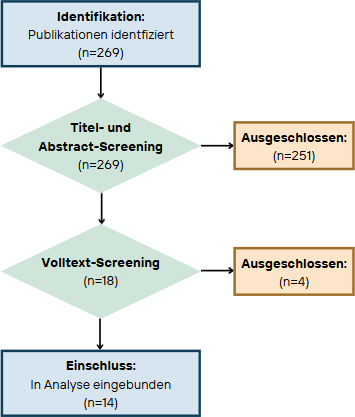
\includegraphics[width=0.5\textwidth]{pictures/SensorDatenFlowchart.png}
            \captionof{figure}{Flussdiagramm des Auswahlprozesses der Paper für die Literaturrecherche zur Integration der Sensordaten.} 
            \label{fig:sensor_flow_chart}
        \end{minipage}
    \end{center}
    \vspace{1ex}

    Die Literatursuche und das anschließende Screening führten zu folgenden Ergebnissen:
    
    In PubMed wurden initial 69 Ergebnisse identifiziert. Nach einem Titel- und Abstract-Screening wurden 10 Publikationen als relevant eingestuft. Das anschließende Volltext-Screening führte zum Ausschluss von zwei weiteren Arbeiten, sodass insgesamt 8 Publikationen aus PubMed in die Analyse einbezogen wurden.
    
    In IEEE Xplore wurden initial 200 Ergebnisse gefunden. Nach dem Titel- und Abstract-Screening verblieben 8 relevante Treffer. Im Zuge des Volltext-Screenings wurden ebenfalls zwei Arbeiten ausgeschlossen, woraus sich 6 finale Publikationen aus IEEE Xplore für die Synthese ergaben.
    
    Die insgesamt $n = 14$ identifizierten Quellen wurden quantitativ analysiert und manuell hinsichtlich der verwendeten Schnittstellenstandards kategorisiert. Der kombinierte Ablauf der Literaturrecherche in PubMed und IEEE Xplore ist im Flussdiagramm in Abbildung \ref{fig:sensor_flow_chart} dargestellt.

    \item[Ergebnisse] 
    Die Analyse zeigt eine deutliche Dominanz des HL7 FHIR Standards, der in $n = 11$ Artikeln Anwendung findet. Lediglich $n = 3$ Quellen setzen auf klassische REST-Schnittstellen zur Datenübertragung.

    \item[Beantwortung] 
    Der Dateneinzug erfolgt primär über den HL7 FHIR Standard oder einfache REST-Schnittstellen. Bemerkenswert ist, dass keine der untersuchten Arbeiten ein kontinuierliches Daten-Streaming in das KIS beschreibt; stattdessen erfolgt die Integration ausschließlich im Batch-Processing-Verfahren durch gezieltes Pulling von den Servern.

\end{description}

\subsubsection{Frage 1.3: Anforderungen an Synthetische Daten}
\begin{description}[style=nextline, font=\bfseries]

    \item[Methodik] 
    Die methodische Grundlage bildet eine systematische Literaturrecherche in den Datenbanken PubMed und IEEE Xplore (Stand: März 2026). Aus den identifizierten Quellen wurden die von den Autoren explizit formulierten Anforderungen manuell extrahiert, um eine ungefilterte Vergleichsbasis für die weiteren Analysen zu schaffen.

    \item[Ergebnisse] 
    Aus den Papern ergaben sich die folgenden Anforderugen:
    \begin{itemize}[leftmargin=1.5em, labelsep=0.5em, itemsep=4pt, topsep=4pt]
    \item \textbf{Statistische Fidelität:} Synthetische Daten müssen die statistischen Eigenschaften des Originaldatensatzes präzise replizieren, insbesondere die Randverteilungen der Variablen und komplexe Korrelationsstrukturen. Hochdimensionale Krankheitskodes sollten dabei eine Korrelation der Kodewahrscheinlichkeiten von R2>0,9 erreichen. \citep{chen_generating_2025} \citep{theodorou_synthesize_2023}
    
    \item \textbf{Strukturelle Integrität:} Es wird eine hierarchische Konsistenz über multiple Tabellen hinweg gefordert (z. B. zwischen Patientenstammdaten und Laborwerten). Zudem müssen klinisch bedeutsame Fehlwerte (Informative Missingness) explizit modelliert werden.\citep{josling_novel_2026}
    
    \item \textbf{Temporale Dynamik:} Bei longitudinalen Daten müssen sowohl die sequenziellen Abhängigkeiten klinischer Ereignisse als auch die spezifischen Zeitintervalle (Inter-visit Gaps) realistisch abgebildet werden. \citep{josling_novel_2026} \citep{theodorou_synthesize_2023}
    
    \item \textbf{Klinische Nutzbarkeit (Utility):} Die Daten müssen im "Train-Synthetic-Test-Real" (TSTR) Framework validiert werden, um sicherzustellen, dass auf synthetischen Daten trainierte Modelle auf realen Daten performant sind. In spezialisierten Domänen wie der Kardiologie wird zudem eine klinische Kohärenz und medizinische Relevanz gefordert, die durch Fachexperten validiert wurde. \citep{theodorou_synthesize_2023} \citep{jung_clinical_2025}
    
    \item \textbf{Datenschutz und Sicherheit:} Eine zentrale Anforderung ist die Vermeidung von Overfitting, um Re-Identifizierungsrisiken zu minimieren. Hierfür wird oft die Integration von Differential Privacy (DP) und die Messung der $\epsilon$-Identifizierbarkeit gefordert. \citep{tsao_health_2023} \citep{hahn_contribution_2022} \citep{chen_generating_2025}
    
    \item \textbf{Governance und Ethik:} Die Generierung sollte den FAIR-Prinzipien (Findable, Accessible, Interoperable, Reusable) entsprechen. Bei der Verwendung von Daten marginalisierter Gruppen müssen zudem die CARE-Prinzipien (Collective benefit, Authority to control, Responsibility, Ethics) beachtet werden. \citep{tsao_health_2023}
    
    \item \textbf{Bias-Vermeidung:} Die Generierungsprozesse dürfen bestehende algorithmische Biases aus den Originaldaten nicht verstärken oder perpetuieren. \citep{theodorou_synthesize_2023}
    \end{itemize}

    \item[Beantwortung] 
    Zusammenfassend lassen sich die in der Literatur formulierten Anforderungen in sieben Kernbereiche unterteilen: statistische Fidelität, strukturelle Integrität, temporale Dynamik, klinische Nutzbarkeit, Datenschutz, Governance/Ethik sowie die aktive Bias-Vermeidung.

\end{description}

% --- ZIEL 2 ---
\subsection*{Ziel 2: Definition der Qualitätskriterien}

\subsubsection{Frage 2.1: Befragung von Expert*innen}

\begin{description}[style=nextline, font=\bfseries]

    \item[Methodik] 
    Zur Erhebung der Expertenanforderungen wurde im ersten Schritt ein strukturierter Gesprächsleitfaden konzipiert. Dieser diente als methodische Grundlage für die anschließenden Experteninterviews und fokussierte sich gezielt auf die medizinische, informationstechnische sowie didaktische Qualität der synthetisch generierten Patientendaten und der in das Lehre-KIS importierten Sensordaten. 

    Dies sind alle Fragen des Leitfadens: 
    \href{https://github.com/robinhefner/Research-Project/blob/5359f58b92f2480c59e9677c2e41ec0f7c742b21/Gespr%C3%A4chsleitfaden_Qualit%C3%A4tskriterien.pdf}{Leitfaden Qualitätskriterien}
    \\

    \vspace{1em}
    Im Anschluss an die Ausarbeitung des Leitfadens erfolgte die Durchführung der eigentlichen Experteninterviews. Hierbei wurde ein zielgruppenadaptierter Ansatz gewählt, um die Befragung optimal an die jeweilige Fachexpertise der Interviewpartner anzupassen. Dies bedeutet konkret, dass nicht jedem Experten der vollständige Fragenkatalog vorgelegt wurde: Personen mit primär medizinischem Hintergrund wurden nicht zu informationstechnischen Details befragt, ebenso wie technische Experten von den spezifisch medizinischen Qualitätskriterien ausgenommen waren.

    \item[Ergebnisse] 
    Durch den gewählten Ansatz konnten insgesamt sechs qualitative Interviews erfolgreich realisiert werden. Die Kohorte der Befragten setzte sich aus drei Personen mit medizinischem Hintergrund sowie drei Person mit informationstechnischer Spezialisierung zusammen. Ein essenzielles Auswahlkriterium, das fünf Experten erfüllten, war ihre ausgewiesene praktische Erfahrung im Bereich der akademischen Lehre. Die Befragung lieferte umfassende, protokollierte Datenbasen für die anschließende Auswertung.

    \item[Beantwortung] 
    Die Befragung der Expert*innen wurde erfolgreich über sechs qualitative, zielgruppenadaptierte Interviews auf Basis eines dreigeteilten Leitfadens (Medizin, IT, Didaktik) durchgeführt. Dadurch konnte ein breites, interdisziplinäres Spektrum an praktischer Lehrerfahrung für die nachfolgende Kriterienauswertung erfasst werden.

\end{description}

\subsubsection{Frage 2.2: Analyse der Ergebnisse: Welche Anforderungen haben Spezialisten an die Daten?}

\begin{description}[style=nextline, font=\bfseries]

    \item[Methodik] 
    Die methodische Auswertung der erhobenen Daten erfolgte über eine qualitative Analyse der zuvor angefertigten Interviewprotokolle. Ziel dieser Analyse war es, die Aussagen der Experten systematisch zu strukturieren, Gemeinsamkeiten zu identifizieren und daraus die übergeordneten Kernanforderungen an die Datenqualität abzuleiten.

    \item[Ergebnisse] 
    Die qualitative Analyse der Interviewprotokolle führte zur Identifikation von vier primären Hauptkriterien für die Datenqualität:
    \begin{enumerate}
        \item \textbf{Klinische Plausibilität:} Beschreibt das medizinisch logische Zusammenspiel von Symptomen, Diagnosen und Behandlungen. Das Spektrum reicht dabei von fehlerfreien Standardtherapien bis zu plausiblen Fehlbehandlungen.
        \item \textbf{Longitudinale Konsistenz:} Bezieht sich auf den langfristigen, korrekten Krankheitsverlauf über größere Zeiträume hinweg. Chronische Erkrankungen und Folgeuntersuchungen müssen lückenlos aufeinander aufbauen und dürfen keine unlogischen Sprünge aufweisen.
        \item \textbf{Zeitlich logische Abfolge:} Umfasst die korrekte Reihenfolge sowie die Realitätsnähe der zeitlichen Abstände einzelner klinischer Ereignisse (z.\,B. die Zeitspanne von der Erstdiagnose über die Intervention bis zur Nachsorge).
        \item \textbf{Gesamteindruck:} Aggregiert die vorgenannten Aspekte zu einem globalen Qualitätseindruck der Patientenakte, welcher maßgeblich die Akzeptanz und den didaktischen Nutzwert für die Studierenden bestimmt.
    \end{enumerate}

    \item[Beantwortung] 
    Die Spezialisten stellen insgesamt vier zentrale Anforderungen an die synthetischen Patientendaten: klinische Plausibilität, longitudinale Konsistenz, eine zeitlich logische Abfolge sowie einen stimmigen Gesamteindruck. Diese extrahierten Kernkriterien definieren die qualitativen Mindestanforderungen, die für eine erfolgreiche und akzeptierte Nutzung in der akademischen Lehre erfüllt sein müssen.

\end{description}

% --- ZIEL 3 ---
\subsection*{Ziel 3: Prototypische Implementierung}
\subsubsection{Frage 3.1: Generierung mittels Synthea}
\begin{description}[style=nextline, font=\bfseries]

    \item[Methodik] 
    Die Patientengenerierung erfolgte auf Basis des öffentlichen Synthea-Repositorys unter Einbeziehung der offiziellen Wiki-Dokumentation zur Modellierung klinischer Abläufe.

    \item[Hürden] 
    Im Implementierungsprozess wurden drei zentrale Herausforderungen adressiert: 
    \begin{itemize}[leftmargin=1.5em, labelsep=0.5em, itemsep=4pt, topsep=4pt]
        \item \textbf{Herkunft der Patienten:}
        Synthea generiert standadtmäßig Patienten die in den USA verortet sind. Das bedeutet im amerikanischen Gesundheitssystem behandelt werden und amerikanische Namen und Adressen besitzen. Die Lösung war es das Repository zu forken (Ein Fork ist eine Kopie eines Repositories, welches den selben Code und Sichtbarkeit besitzt wie das ursprüngliche Repository) und die EU/DE Properties, die von Synthea zur Verfügung gestellt werden zu nutzen und eigene Änderungen einzuführen um Patienten die in der EU / Deutschland verortet werden zu erhalten.
        Durch die zur Verfügung gestellten Properties von Synthea wurden Krankenhäuser, sowie Städte und Krankenkassen aus deutschland importiert. Die Änderungen die nachträglich noch erstellt wurden waren die Einführung deutscher Vor und Nachnamen, sowie deutscher Straßennamen, welche in Synthea auch synthetisch generiert werden.
        \item \textbf{Vorgenerierung einer kompletten Patientenhistorie:}
        Synthea erstellt für einen Patienten immer eine komplette lückenlose Patientnehistorie. Das bedeutet, dass von Geburt bis ggf. Tod die Geschichte eines Patienten erstellt wird. Für eine möglichst realistisches KIS ist dies jedoch wenig repräsentativ. Als Lösung haben wir hierfür die FHIR Bundle, die von Synthea erstellt werden in einzelne Transaktionen aufgeteilt. Hierdurch kann die Patientenhistorie aufgeteilt werden und nur bis zu einem bestimmten Punkt ins KIS importiert werden. Wie dies gestaltet werden soll, also bis zu welchem Punkt die Daten importiert werden und wo der Cut-Off gesetzt wird steht noch offen.
        \item \textbf{Ärzte in Synthea und der Umgang im KIS:}
        Synthea erstellt für einen Patienten immer eine Liste an Ärzten, die diesen über den Verlauf behandelt haben. Dies würde für das studiKIS bedeuten, das sich die Menge der Ärzte exponentiell erhöhen würde, da jeder Patient eine Vielzahl an Ärzten hat die ihn im Verlauf behandeln. Ein Lösungsansatz wird in den Ergebnissen zu Frage 3.c dargestellt.
    \end{itemize}

    \item[Ergebnisse] 
    Es wurde ein funktionsfähiger Workflow etabliert, der die bedarfsgerechte Erzeugung beliebig großer Patientenkollektive im standardisierten FHIR-Format ermöglicht.

    \item[Beantwortung] 
    Durch die gezielte Anpassung des Synthea-Frameworks und die Implementierung regionaler Spezifika konnte eine Pipeline geschaffen werden, die lokalisierte und prozessual steuerbare synthetische Patientendaten für die Systemintegration bereitstellt.

\end{description}

\subsubsection{Frage 3.2: Generierung mittels LLM} 
\textbf{Methodik:} Entwicklung eines Prompts, der es ermöglicht strukturierte klinische Daten als FHIR Bundle zu erzeugen. \\
\textbf{Hürden:} 
\begin{itemize}
    \item \textbf{Halluzination von Krankheiten:} Eine Hürde war es, dass bei der Generierung der Daten vom LLM Verläufe halluziniert wurden die nicht konsistent waren und wenig Plausibel. Hierfür wurde als Lösungsansatz eine Liste an Diagnosen und Medikamenten dem LLM zur Verfügung gestellt. Hierdurch wurden plausiblere und konsistentere Daten erzeugt.
    \item  \textbf{Inkonsistenz im Format:} Bei der Erzeugung von FHIR Bundlen im json Format traten inkonsistenzen in der Formatierung auf. Durch erweiterung des Prompt mit Punkt 6. OpenMRS-Kompatibilität  und 7. Formatvorgabe konnte dies überwunden werden. 
\end{itemize}

\textbf{Ergebnisse:} Mithilfe des erstellten Prompts können durch die Nutzung von des Modells Gemini 3.1 Pro (High) \\

Link zum Prompt:
\href{https://github.com/robinhefner/Research-Project/blob/9ac45330eabbaa19dd4e6c5fe2f43b0358648f0d/Prompt_FHIR_Datengenerierung.md}{Prompt FHIR Datengenerierung}
\\


\textbf{Beantwortung:} Durch einen Prompt der dem Modell klare Richtlinien gibt können Patientendaten im FHIR Format erstellt werden.\\


\subsubsection{Frage 3.3: Import der Daten ins KIS}

\begin{description}[style=nextline, font=\bfseries]

    \item[Methodik] 
    Der Import der generierten Patientendaten in das bestehende Lehre-KIS erfolgte über die integrierte FHIR-Schnittstelle.

    \item[Hürden] 
    Im Rahmen des Importprozesses traten mehrere technische Herausforderungen auf:
    
    \begin{itemize}[leftmargin=1.5em, labelsep=0.5em, itemsep=4pt, topsep=4pt]
        \item \textbf{Fehlende Dokumentation:} Eine wesentliche Erschwerung stellte die unzureichende Dokumentation des FHIR-Moduls von Bahmni dar. Die korrekten Formate und Endpunkte für den Import spezifischer klinischer Informationen der generierten Patientendaten (wie Diagnosen und Medikation) mussten empirisch ermittelt werden.
        
        \item \textbf{Fehlende Concept Mappings:} Die von Synthea generierten Patientendaten enthielten Diagnosecodes, die standardmäßig nicht in Bahmni hinterlegt waren. Dieses Problem konnte durch die Integration des CIEL-Concept-Dictionaries (Columbia International eHealth Laboratory) gelöst werden.
        
        \item \textbf{Neu generierte Ärzte:} Ein weiteres signifikantes Hindernis beim Importprozess stellte die Handhabung des medizinischen Personals dar. Synthea generiert standardmäßig nicht nur die eigentlichen klinischen Patientendaten, sondern verknüpft diese systematisch mit eigens dafür neu erstellten, virtuellen Behandlern. Um einen erfolgreichen Import zu gewährleisten, hätte dies bedeutet, dass für jeden neuen Datensatz zwingend auch das jeweils neu generierte ärztliche Personal im Lehre-KIS angelegt werden müsste. Da sich Synthea systemseitig nicht so konfigurieren lässt, dass es auf einen vordefinierten, fixen Pool an Ärzten zurückgreift, würde dieser Umstand bei fortlaufender Datengenerierung zu einem exponentiellen und unkontrollierbaren Anwachsen des Arztstamms in der Systemdatenbank führen. Um dieser Problematik zu begegnen, sollte ein dezidiertes Skript entwickelt werden. Dieses durchsucht das von Synthea erzeugte FHIR-Bundle automatisiert nach den verknüpften Behandlern und ersetzt diese systematisch durch eine vordefinierte Auswahl real existierender Ärzte aus dem Lehre-KIS. Um die Konsistenz zu wahren, wurden hierbei exakt dieselben fünf Fachabteilungen beziehungsweise ärztlichen Rollen verwendet (Kardiologie, Neurologie, Chest Pain Unit, Stroke Unit, Neurologische Reha), die zuvor auch dem Large Language Model (LLM) als Kontext für die Generierung der Patientendaten übergeben wurden. Aufgrund von zeitlichen Enschränkungen wurde das Skript final jedoch nicht entwickelt, es wurde lediglich Daten für einen Probepatient erstellt, bei dem die meisten Einträge der Synthea generierten Daten entfernt und bei den bleibenden Observations der Behandler ersetzt wurde. 
        
        \item \textbf{Komplexe Synthea-Datenstruktur:} Selbst nach dem erfolgreichen Mapping fehlender klinischer Konzepte und der Ersetzung der Behandler bei den Daten des Probepatienten traten beim Import weiterhin gravierende Kompatibilitätsprobleme auf. Die generierten Patientendaten enthielten spezifische FHIR-Ressourcen und Datenfelder, die von der Architektur des Lehre-KIS abgelehnt wurden. Um diese Inkompatibilitäten aufzulösen, wurde zunächst ein iterativer Ansatz verfolgt: Die Datensätze wurden eingelesen, der resultierende Error-Log analysiert, das fehlerverursachende Feld im Skript entfernt und der Importprozess wiederholt. Obwohl das Skript dahingehend erweitert wurde, betroffene Felder sukzessive zu bereinigen, stieß dieser Ansatz auf weitere Hürden. Es traten kontinuierlich neue Fehler auf, beispielsweise durch klinische Konzepte, die selbst durch das zuvor implementierte CIEL-Mapping nicht abgedeckt waren. Eine theoretische Lösung hätte in der Erweiterung des Einleseskripts bestanden, sodass dieses fehlende Konzepte dynamisch im Lehre-KIS anlegt und mit den Codes aus dem Synthea-FHIR-Bundle verknüpft. Angesichts strikter zeitlicher Restriktionen und der hohen technischen Komplexität wurde dieser Pfad jedoch verworfen, und der Fokus wurde vollständig auf den korrekten Import der durch das LLM generierten Patientendaten gelegt. Der Versuch, die Synthea-Datensätze durch kontinuierliches Entfernen von Feldern anzupassen, erwies sich letztlich als nicht ausreichend skalierbar: Bei jedem neuen Generierungslauf hätten potenziell neue, bislang unbekannte Felder auftreten können, die das Einleseskript noch nicht abfängt und die unweigerlich zu neuen Fehlimporten geführt hätten. Letztlich war dieses ressourcenintensive Vorgehen jedoch der unzureichenden Dokumentation des Bahmni-FHIR-Moduls geschuldet, da im Vorfeld nicht spezifiziert war, welche Felder in welcher Formatierung zwingend erwartet oder strikt abgelehnt werden.
        
        \item \textbf{Darstellung der Laborwerte:} Die Abbildung von Laborwerten in Bahmni erfordert regulär einen zweistufigen Prozess (Order-Anforderung und LIS-Rückmeldung), um im Dashboard als dediziertes „Labor Ergebnis“ zu erscheinen. Die Nachbildung dieses spezifischen FHIR-Objekts für die generierten Patientendaten erwies sich als nicht zielführend. Die Replikation der Struktur eines manuell angelegten Laborwerts führte beim Import lediglich zur Erstellung einer allgemeinen Observation.
    \end{itemize}

    \item[Ergebnisse] 
    Aufgrund der anfänglich unzureichenden Dokumentation der FHIR - Schnittstelle wurde initial ein Skript entwickelt, das den manuellen Erstellungsprozess von Laborwerten über die grafische Benutzeroberfläche von Bahmni simuliert. Hierfür wurde systematisch analysiert, welche URLs bei den jeweiligen Interaktionen in der UI aufgerufen und welche Datenobjekte dabei übermittelt wurden. Diese Netzwerkinformationen wurden extrahiert und algorithmisch im Skript repliziert. Es gelang, nahezu den gesamten Prozess ausschließlich über diese nachgebildeten HTTP-Anfragen abzubilden. Eine Ausnahme bildete lediglich der Schritt, bei dem die ID des Laborauftrags  mit der ID der Patientendaten verknüpft wird. Diese Verknüpfung wird bei der manuellen Eingabe nicht explizit als separates Datenpaket gesendet, sondern beim dynamischen Seitenaufbau des Laborinformationssystems direkt in die anklickbaren URLs eingebettet. Um diese zwingend notwendige Verbindung programmtechnisch zu extrahieren, musste als Workaround auf eine direkte SQL-Abfrage der zugrunde liegenden Datenbank zurückgegriffen werden. Mithilfe dieses Skripts war es anschließend möglich, automatisiert eine Vielzahl von Laborwerten zu den jeweiligen Patientendaten hinzuzufügen, ohne die zeitaufwendigen manuellen Schritte in der UI durchlaufen zu müssen. Ein entscheidender Nachteil dieser Methode war jedoch, dass sich die Laborwerte auf diese Weise nicht mit historischen Zeitstempeln versehen ließen. 
    
    Aus diesem Grund wurde der Fokus im darauffolgenden Schritt erneut auf die Realisierung des Imports über die reguläre FHIR-Schnittstelle gelegt. Durch umfangreiche empirische Analysen und iteratives Testen konnte schließlich das exakte FHIR-Schema identifiziert werden, das vom Lehre-KIS fehlerfrei akzeptiert wird. Mit der Kenntnis dieser genauen strukturellen Anforderungen wurde das verwendete LLM mittels spezifischem Prompting angewiesen, die generierten Patientendaten exakt in diesem Format zu erzeugen. Diese Maßnahme führte dazu, dass sich die resultierenden Patientendaten problemlos in das System einlesen ließen.
    
    Nachdem auch die korrekte FHIR-Datenstruktur für die Laborwerte ermittelt war, konnten diese ebenfalls über die Schnittstelle importiert werden. Einschränkend muss hierbei erwähnt werden, dass die Laborwerte systembedingt stets als Teil einer allgemeinen „Observation“ eingelesen wurden und nicht als dedizierte „Labor Ergebnisse“ in der nativen Kategorie des Systems persistiert werden konnten. Da sich diese Observationen jedoch problemlos und historisch korrekt im Trends-Dashboard visualisieren ließen, in welchem die Laborwerte im zeitlichen Verlauf dargestellt werden, wurde diese Art der Abspeicherung für die Zwecke des Projekts als vollkommen ausreichend erachtet.

    \item[Beantwortung] 
    Zusammenfassend lässt sich feststellen, dass der Import generierter Patientendaten über die FHIR-Schnittstelle in das Lehre-KIS erfolgreich realisierbar ist, sofern die Datensätze exakt der identifizierten, systemspezifischen FHIR-Struktur entsprechen.

\end{description}
\subsubsection{Frage 3.4: Dynamischer Datenimport}
\textbf{Methodik:} Import der Daten über einen zeitlichen Verlauf um realitätsnahe zeitliche Verläufe abzublilden. \\
\textbf{Ergebnisse:} Die synthetisch generierten Daten werden mithilfe eines Python-Scripts in einzelne FHIR Transaktionen aufgeteilt, die in einer SQLite Datenbank abgespeichert werden. Die Transaktionen besitzen neben den FHIR Daten eine Scheduled-Time zu der sie im KIS vorhanden sein sollen. Ein zweites Script, welches auf dem KIS-Server als Cronjob (Ein Cronjob wird zu einem definierten Zeitpunkt regelmäßig ausgeführt) läuft importiert die Einträge aus der Datenbank in das KIS bei denen die planmäßige Zeit erreicht wurde.\\
\textbf{Beantwortung:}


% --- ZIEL 4 ---
\subsection*{Ziel 4: Bewertung der Ansätze}
\subsubsection{Frage 4.1: Auswahl der Datenquellen}
\begin{description}[style=nextline, font=\bfseries]
    \item[Methodik] Für die Evaluierung werden Daten aus agentenbasierten und nicht-agentenbasierten Systemen, sowie reale Patientendaten herangezogen. Diese Datensätze werden anschließend durch medizinisches Fachpersonal anhand der in Ziel 2 definierten Kriterien bewertet.
    \item[Ergebnisse] Als nicht-agentenbasiertes System wird das Framework Synthea zur Generierung synthetischer Patientendaten genutzt. Die agentenbasierten Daten werden durch Large Language Model erzeugt. Ergänzend werden reale, anonymisierte Patientendaten aus dem MIMIC-III-Datensatz integriert. Es wurde eine gleichmäßige Verteilung (40/40/40-Split) gewählt, sodass sich eine Gesamtstichprobe von 120 Datensätzen für die Bewertung ergibt.
    \item[Beantwortung] Die Auswahl der Datenquellen deckt somit drei Dimensionen ab: agentenbasierte LLM-Generierung, regelbasierte Synthea-Simulation und reale klinische Daten aus MIMIC-III.
\end{description}

\subsubsection{Frage 4.2: Einheitliches Darstellungsformat}
\begin{description}[style=nextline, font=\bfseries]

    \item[Methodik] 
    Um eine objektive und unverzerrte Evaluation aller Datensätze durch die Gutachter zu gewährleisten, mussten die Patientendaten in einem einheitlichen und standardisierten Format präsentiert werden. Ursprünglich war vorgesehen, die Visualisierung direkt über das Lehre-KIS zu realisieren. Da sich das Einlesen der Synthea-Patientendaten in das Lehre-KIS jedoch als nicht durchführbar erwies, musste eine alternative Darstellungsmethode evaluiert werden. Die direkte Verwendung der rohen FHIR-Daten wurde umgehend verworfen, da eine manuelle Sichtung und Plausibilitätsprüfung von teils über 60.000 Zeilen FHIR-Code für die medizinischen Experten im Rahmen einer Evaluation nicht praktikabel ist. Schließlich wurde entschieden, die Patientendaten im PDF-Format aufzubereiten, da dies die zugänglichste und universellste Option für alle Beteiligten darstellte.

    \item[Hürden] 
    Der Prozess der Formatvereinheitlichung war mit mehreren technischen Herausforderungen verbunden. Das Framework Synthea verfügt über keinen nativen PDF-Export. Die integrierte Option eines HTML-Exports führte im lokalen Systemkontext zu Fehlern. Ebenso scheiterten Versuche, die von Synthea generierten FHIR-Dateien über webbasierte Plattformen wie \textit{clinFHIR} oder den \textit{HAPI-FHIR-Server} adäquat zu visualisieren. Als verbleibende Alternative wurde der CSV-Export von Synthea genutzt. Es wurde ein proprietäres Skript entwickelt, das die exportierten CSV-Strukturen einliest und daraus ein übersichtliches PDF-Dokument generiert, welches alle demografischen und klinischen Parameter abbildet.

    Im nächsten Schritt mussten die übrigen Datensätze, bestehend aus den anonymisierten Musterelementen der Datenspende sowie den vom LLM generierten FHIR-Dateien, in exakt dieselbe CSV-Struktur überführt werden. Hierzu wurde ein zweites Skript implementiert, welches auf Basis der heterogenen FHIR-Eingangsdaten strukturell identische CSV-Tabellen erzeugt. Durch diese Standardisierung konnten im anschließenden Schritt mithilfe des primären Generierungsskripts für alle drei Datenquellen optisch und strukturell ununterscheidbare PDFs erzeugt werden.

    Eine spezifische Hürde bei den Musterschulungsdaten lag in deren vollständiger Anonymisierung: Alle Datensätze wiesen identische Personennamen auf und enthielten keinerlei Adressdaten. Um zu verhindern, dass die Evaluatoren allein anhand dieser demografischen Leerstellen auf die Gruppenzugehörigkeit der Patientendaten schließen können, wurden die Datensätze algorithmisch mit pseudozufälligen Klarnamen und Adressen angereichert. Dabei wurde das im Originaldatensatz hinterlegte biologische Geschlecht berücksichtigt, um durch passende Vornamen logische Inkonsistenzen und damit verbundene Verzerrungen bei der Bewertung auszuschließen.

    Zudem unterschieden sich die Datenquellen erheblich in ihrer Informationstiefe. Die Synthea-Datensätze enthielten komplexe Zusatzinformationen wie Versicherungsverhältnisse, Abrechnungsmodalitäten und detaillierte Pflegepläne, welche weder in den LLM-Daten noch in den Musterelementen der Datenspende existierten. Um strukturelle Diskrepanzen zu eliminieren, wurde der Anzeigeumfang in den PDF-Dokumenten vereinheitlicht. Neben den demografischen Stammdaten wurden restriktiv nur die folgenden fünf klinischen Kategorien aggregiert und dargestellt: „Allergien“, „Diagnosen“, „Medikamente“, „Behandlungen“ sowie „Labor- \& Vitalwerte“.

    \item[Ergebnisse] 
    Als zentrales Artefakt resultieren zwei Skripte: Das erste Skript transformiert die LLM-generierten sowie die realen FHIR-Datensätze in standardisierte CSV-Strukturen, während das zweite Skript diese Tabellen in das finale PDF-Layout konvertiert. Auf diese Weise wurden insgesamt 120 standardisierte PDF-Dokumente erzeugt, jeweils 40 Datensätze pro Kategorie. Diese einheitliche Aufbereitung ermöglicht den Gutachtern eine effiziente, vergleichende Analyse der klinischen Inhalte.

    \item[Beantwortung] 
    Mithilfe der eigens entwickelten Transformationsskripte ist es gelungen, Patientendaten aus drei technologisch unterschiedlichen Quellen so zu harmonisieren, dass sie rein visuell nicht voneinander zu unterscheiden sind. Das finale PDF-Format ist zudem so reduziert und übersichtlich gestaltet, dass medizinische Experten ohne FHIR-Anwenderkenntnisse eine valide qualitative Bewertung der synthetischen Krankengeschichten vornehmen können.

\end{description}

\subsubsection{Frage 4.3: Effiziente Durchführung der Evaluierung}
\begin{description}[style=nextline, font=\bfseries]
\item[Methodik] Zur Durchführung der Evaluierung muss eine intuitive Infrastruktur geschaffen werden, die sowohl die Visualisierung der Patientendaten als auch die Datenerfassung effizient abbildet. Für die Kriterien wird eine 5-stufige Likert-Skala sowie ein optionales Freitextfeld für qualitatives Feedback festgelegt. Um die Validität der Ergebnisse zu gewährleisten, muss das System sicherstellen, dass jede bewertende Person jeden Datensatz exakt einmal evaluiert, um Mehrfachbewertungen auszuschließen. Zudem ist eine kontinuierliche Datenpersistenz notwendig, um Datenverlust zu jedem Zeitpunkt der Erhebung auszuschließen.

\item[Ergebnisse] Als Lösung für die definierten Anforderungen wurde eine passwortgeschützte, webbasierte Anwendung implementiert (\href{https://eval.rhefner.de/}{Link: Evaluierungsplattform}). Um Verzerrungen (Bias) zu minimieren, wurden drei anonymisierte Bewertungsprofile angelegt, deren Zuweisung an die Mediziner durch eine externe Person randomisiert und verblindet erfolgte. Zur Unterstützung der Evaluierenden und zur Gewährleistung eines standardisierten Ablaufs wurde eine schriftliche Anleitung erstellt und den Medizinern bereitgestellt (\href{https://github.com/robinhefner/Research-Project/blob/5359f58b92f2480c59e9677c2e41ec0f7c742b21/Anleitung_Evaluation.pdf}{Link: Anleitung Evaluation}). Die Benutzeroberfläche wurde zweigeteilt gestaltet: Auf der linken Seite wird ein zufällig ausgewählter, noch unbewerteter Patientendatensatz als PDF dargestellt, während auf der rechten Seite die zugehörigen Likert-Skalen und Textfelder platziert sind. Nach dem Absenden einer Bewertung werden die Daten direkt in einer Cloud-Datenbank persistent gespeichert. Das System filtert nach jedem Durchgang die bereits bewerteten Fälle und lädt dynamisch den nächsten unbewerteten Datensatz, bis alle 120 Datensätze vollständig abgearbeitet sind. Der Prozess schließt mit einer Bestätigungsmeldung über den erfolgreichen Abschluss ab.

\item[Beantwortung] Die Anforderungen an eine strukturierte, persistente und fehlerfreie Datenerhebung wurden durch die Entwicklung einer passwortgeschützten Webanwendung realisiert. Diese ermöglicht über ein zweigeteiltes Interface die Evaluierung mittels Likert-Skalen, schließt Mehrfachbewertungen systemseitig aus und sichert den Fortschritt der Bewertenden kontinuierlich in einer Cloud-Datenbank. Eine begleitende Anleitung stellte zudem die Standardisierung des Bewertungsprozesses sicher.
\end{description}

\subsubsection{Frage 4.4: }
\begin{description}[style=nextline, font=\bfseries]

    \item[Methodik] 

    \item[Hürden] 

    \item[Ergebnisse] 


    \item[Beantwortung] 
\end{description}
\begin{landscape}
\section{Zeitplan}
\begin{landscape}
\begin{center}
\resizebox{\linewidth}{!}{
\begin{ganttchart}[
    hgrid,
    vgrid,
    time slot format=isodate,
    title/.style={fill=gray!10},
    title label font=\footnotesize,
    canvas/.style={draw=black, fill=white},
    bar height=0.6,
    group height=0.7,
    milestone height=0.6,
    bar/.append style={rounded corners=2pt},
    group/.append style={rounded corners=2pt, draw=black, fill=gray!20},
    milestone/.append style={fill=black},
    x unit=0.25cm, % Kleinerer Wert, damit der lange Zeitraum auf die Seite passt
    y unit chart=0.7cm
]{2026-02-23}{2026-06-14}

% Title - Die Zahlen am Ende müssen zur Gesamtzahl der Tage passen
\gantttitle{Projektzeitplan Research-Project}{105} \\
\gantttitlecalendar{month=name, week} \\ % 'week' statt 'day' spart extrem viel Platz!

% Section: Recherche
\ganttgroup{Recherche}{2026-02-23}{2026-05-11} \\
\ganttbar[bar/.append style={fill=research}]{AP1 Literatur}{2026-02-23}{2026-03-20} \\
\ganttbar[bar/.append style={fill=research!70}]{AP2 Kriterien}{2026-03-21}{2026-05-11} \\

% Section: Entwicklung
\ganttgroup{Entwicklung}{2026-03-21}{2026-05-17} \\
\ganttbar[bar/.append style={fill=development}]{AP3 Implementierung}{2026-03-21}{2026-05-17} \\

% Section: Abschluss
\ganttgroup{Abschluss}{2026-05-18}{2026-05-31} \\
\ganttbar[bar/.append style={fill=closure}]{AP4 Bewertung}{2026-05-18}{2026-05-31} \\

% Section: Artikel
\ganttgroup{Artikel}{2026-03-02}{2026-06-14} \\
\ganttbar[bar/.append style={fill=article}]{Wissenschaftlicher Artikel}{2026-03-02}{2026-06-14}

\end{ganttchart}
}
\end{center}
\end{landscape}
\end{landscape}
\end{document}